Assuming that input has been appropriately treated to eliminate redundant
features, we may turn to characterise proposed surrogate models and the criteria
used for their evaluation. The task all presented surrogates strive to solve can be
formulated using the language of conventional regression problems. In the scope
of this work, we explore various possible choices available to us in the
scheme of supervised and unsupervised learning.

Labeling the expensive Monte Carlo simulation $f(x)$, a surrogate is a mapping
$\hat{f}(x)$ that yields similar images as $f(x)$. In other words, $f(x)$ and
$\hat{f}(x)$ minimise a selected similarity metric. Furthermore, in order to
be considered \textit{viable}, surrogates are required to achieve expected evaluation time
that does not exceed the expected evaluation time of $f(x)$.

In the supervised learning setting, we first gather a sufficiently large
training set of samples $\mathcal{T}=\left\{\left( x^{(i)},f\left(x^{(i)}\right) \right)\right\}_{i=1}^N$
to describe the behaviour of $f(x)$ across its domain.
Depending on specific model class and appropriate choice of its
hyperparameters, surrogate models $\hat{f}(x)$ are trained to minimise
empirical risk with respect to $\mathcal{T}$ and a model-specific
loss function $\mathcal{L}$, where empirical risk is defined as
$R_{\text{emp.}}(\hat{f}\mid\mathcal{T},\mathcal{L})
	=\frac{1}{N}\sum_{i=1}^N
	\mathcal{L}\left(\hat{f}(x^{(i)}),f(x^{(i)})\right)$.


The unsupervised setting can be viewed as an extension of this method.
Rather than fixing the training set $\mathcal{T}$ for the entire duration of
training, multiple sets $\{\mathcal{T}_k\}_{k=0}^K$ are used, such that
$\mathcal{T}_{k-1}\subset\mathcal{T}_k$ for all $k>1$. The first set
$\mathcal{T}_0$ is initialised randomly to provide a \textit{burn-in}, and is
repeatedly extended in epochs, whereby each epoch trains a new surrogate on
$\mathcal{T}_k$ using the supervised learning procedure, evaluates its
performance, and forms a new set $\mathcal{T}_{k+1}$ by adding more samples to
$\mathcal{T}_k$. This permits the learning algorithm to condition the selection
of new samples by the results of evaluation in order to focus on improvement of
surrogate performance in complex regions within the domain.


\subsection{Metrics}
\label{sec:metrics}

Aiming to provide objective comparison of a diverse set of surrogate model
classes, we define a multitude of metrics to be tracked during experiments.
Following the motivation of this work, two desirable properties of surrogates
arise: (i) their capability to approximate the expensive
model well and (ii) their time of evaluation. An ideal surrogate would maximise
the former while minimising the latter.

\Cref{tbl:metrics} provides exhaustive listing and description of metrics recorded
in the experiments. For regression performance analysis, we include a selection
of absolute metrics to assess the approximation capability of surrogates, and set
practical bounds on the expected accuracy of their predictions. In addition, we also track
relative measures that are better-suited for model comparison between works as
they maintain invariance with respect to the selected domain and image space.
For analysis of evaluation time, surrogates are assessed in terms of wall time
elapsed during training and predicition. This closely models the practical use
case, in which they are trained and used as drop-in replacements for the
expensive model. Since training set sizes remain to be determined, all times are
reported per a single sample. Even though some surrogates support acceleration
by means of parallelisation, measures were taken to ensure sequential
processing of samples to achieve comparability between considered models.

\begin{table}[h]
	\centering
	\begin{tabular}{llrl}
	\toprule
	Regression performance metrics	& Mathematical formulation / description &
	\multicolumn{2}{c}{Ideal value} \\
	\midrule
	Mean absolute error (MAE)	& $\sum_{i=1}^N |y^{(i)}-\hat{y}^{(i)}|/N$ & 0
								& [TBR] \\
	Standard error of regression $S$	& $\text{StdDev}_{i=1}^N\left\{ |y^{(i)} -
	\hat{y}^{(i)}| \right\} $	 & 0 & [TBR] \\
	Coefficient of determination $R^2$	& $1-\sum_{i=1}^N \left(y^{(i)}-\hat{y}^{(i)} \right)^2 /
	\sum_{i=1}^N \left( y^{(i)}-\overline{y} \right)^2 $ & 1 & [rel.] \\
	Adjusted $R^2$	& $1-(1-R^2)(N-1)/(N-P-1)$	& 1 & [rel.] \\
	\midrule
	Evaluation time metrics	& {} & {} & {} \\
	\midrule
	Mean training time $\overline{t}_{\text{trn.}}$	& $(\text{wall training time of
	$\hat{f}(x)$})/N_0$ 	& 0 & [ms] \\
	Mean prediction time $\overline{t}_{\text{pred.}}$	& $(\text{wall prediction time of
	$\hat{f}(x)$})/N$	& 0 & [ms] \\
	Relative speedup	& $(\text{wall evaluation time of $f(x)$}) /
	(N\overline{t}_{\text{pred.}})$	&
	$\to\infty$ & [rel.] \\
	\bottomrule
	\end{tabular}
	\caption{Metrics recorded in supervised learning experiments. In
	formulations, we work with training set of size $N_0$ and testing set of
size $N$, TBR values $y^{(i)}=f(x^{(i)})$ and $\hat{y}^{(i)}=\hat{f}(x^{(i)})$
denote images of the $i$th testing sample in the expensive model and the surrogate
respectively. Furthermore, the mean $\overline{y}=\sum_{i=1}^N y^{(i)}/N$ and $P$ is the
number of input features.}
	\label{tbl:metrics}
\end{table}

To prevent undesirable bias in results due to training set selection, all metrics
are collected in the scheme of $k$-fold cross-validation with a standard choice of
$k=5$. Herein, a sample set is subdivided into 5 disjoint folds which are
repeatedly interpreted as training and testing sets, maintaining a constant
ratio of samples between the two. In each such interpretation experiments are
repeated, and the overall value of each metric of interest is reported as the
mean across all folds.


\subsection{Supervised Learning Experiments}
\label{sec:supervised}

\subsubsection{Considered Surrogates}

\begin{table}[h]
	\centering
	\begin{tabular}{llll}
	\toprule
	Surrogate & Acronym & Implementation & Hyperparameters \\
	\midrule
	Support vector machines	& SVM & SciKit Learn & TODO \\
	Gradient boosted trees	& GBT & SciKit Learn & TODO \\
	Extremely random trees	& ERT & SciKit Learn & TODO \\
	AdaBoost	& AB & SciKit Learn & TODO \\
	Gaussian process regression	& GPR & SciKit Learn & TODO \\
	$k$ nearest neighbours	& KNN & SciKit Learn & TODO \\
	Neural networks	& NN & Keras (TensorFlow) & TODO \\
	Inverse distance weighing & IDW & SMT & TODO \\
	Radial basis functions & RBF & SMT & TODO \\
	Stochastic gradient descent & SGD & SciKit Learn & TODO \\
	Ridge regression & RR & SciKit Learn & TODO \\
	Kriging & KRG & SMT & TODO \\
	\bottomrule
	\end{tabular}
	\caption{TODO}
	\label{tbl:surrogates}
\end{table}

TODO: describe classes of surrogates

TODO: reference implementations and original papers

TODO: define NN architectures

\begin{figure}[h]
	\centering
	\begin{subfigure}[b]{0.20\textwidth}
		\centering
		{\footnotesize \incfigscale{0.62}{1h3f}}
		\caption{$\text{1h3f}(W)$}
	\end{subfigure}\hfill%
	\begin{subfigure}[b]{0.15\textwidth}
		\centering
		{\footnotesize \incfigscale{0.62}{kf}}
		\caption{$\text{df}(D,W)$}
	\end{subfigure}\hfill%
	\begin{subfigure}[b]{0.15\textwidth}
		\centering
		{\footnotesize \incfigscale{0.62}{3pyramid}}
		\caption{$\text{3pyr}(W)$}
	\end{subfigure}\hfill%
	\begin{subfigure}[b]{0.20\textwidth}
		\centering
		{\footnotesize \incfigscale{0.62}{5diam}}
		\caption{$\text{5diam}(W)$}
	\end{subfigure}\hfill%
	\begin{subfigure}[b]{0.20\textwidth}
		\centering
		{\footnotesize \incfigscale{0.62}{kf}} % TODO
		\caption{$\text{6sym}(W)$}
	\end{subfigure}

	\caption{TODO}
	\label{fig:neural-net-architectures}
\end{figure}

\subsubsection{Experiments}

TODO: single slice hyperparameter optimisation

TODO: multislice (mixed) hyperparameter optimisation

TODO: retraining for scaling benchmark

TODO: retraining on large set


\newpage

\subsection{Adaptive Sampling}
\label{sec:adaptive}

All of the surrogate modelling techniques studied in this project face a shared challenge: their accuracy is limited by the quantity of training samples which are available from the expensive MC model. Adaptive sampling procedures can improve upon this limitation by taking advantage of statistical information which is accumulated during the training of any surrogate model. Rather than training the surrogate on a single sample set generated according to a fixed strategy, sample locations are chosen incrementally so as to best suit the model under consideration.

Adaptive sampling techniques are widespread in the literature and have been specialised for surrogate modelling. Garud's [1] "Smart Sampling Algorithm" achieved notable success by incorporating surrogate quality and crowding distance scoring to identify optimal new samples, but was only tested on a single-parameter domain. We theorised that a nondeterministic sample generation approach, built around Markov Chain Monte Carlo methods (MCMC), would fare better for high-dimensional models by more thoroughly exploring all local optima in the parameter space. MCMC produces a progressive chain of sample points, each drawn according to the same symmetric proposal distribution from the prior point. These sample points will converge to a desired posterior distribution, so long as the acceptance probability for these draws has a particular functional dependence on that posterior value (see [2] for a review). 

Many researchers have embedded surrogate methods into MCMC strategies for parameter optimisation [3][4], in particular the ASMO-PODE algorithm [5] which makes use of MCMC-based adaptive sampling to attain greater surrogate precision around prospective optima. Our novel approach draws inspiration from ASMO-PODE, but instead uses MCMC to generate samples which increase surrogate precision throughout the entire parameter space.

\begin{wrapfigure}{r}{0.5\textwidth}
  \vspace{-35pt}
  \begin{center}
    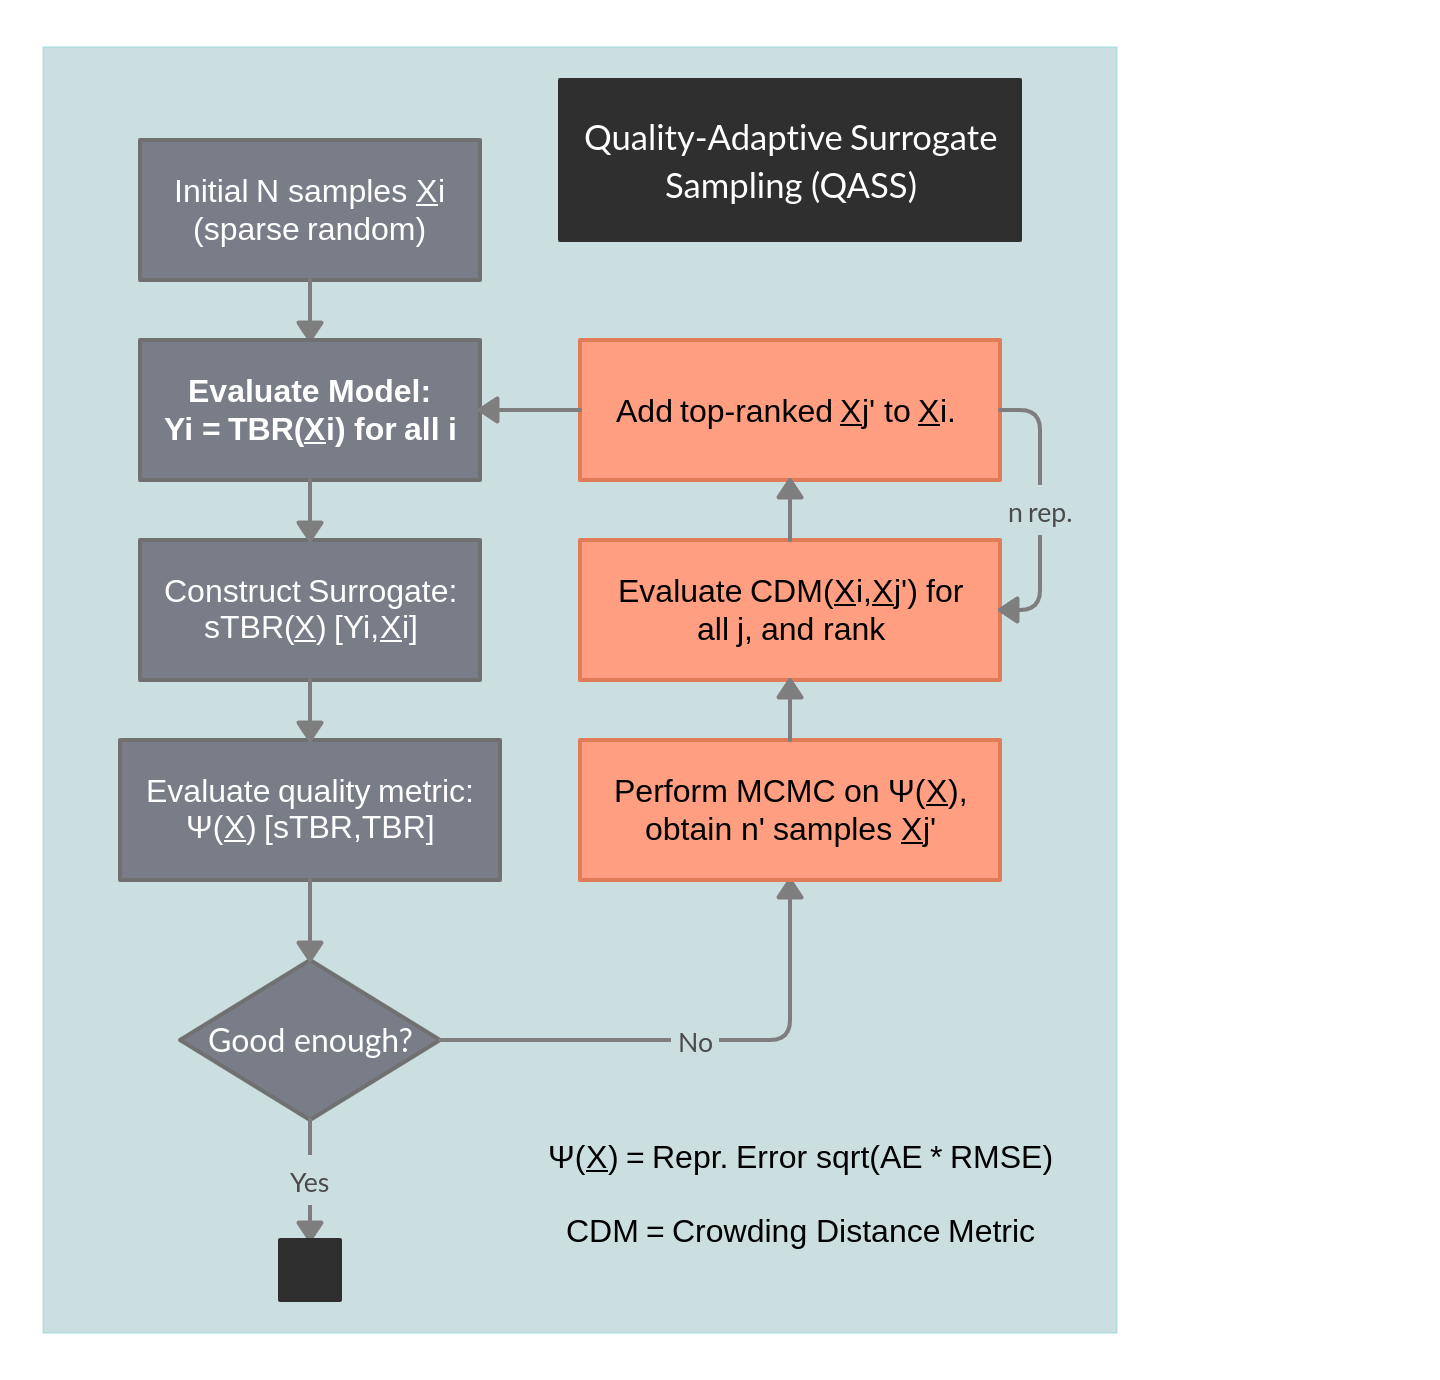
\includegraphics[width=0.6\textwidth]{fig4_qassplan.png}
    \caption{Schematic of QASS algorithm}
    \label{fig:qassplan}
  \end{center}
  \vspace{-20pt}
\end{wrapfigure}

We designed the Quality-Adaptive Surrogate Sampling algorithm (QASS) to iteratively increment the training set with sample points which maximise surrogate error and minimise a crowding distance metric (CDM) [6] in parameter space. On each iteration following an initial training of the surrogate on $N$ uniformly random samples, test error values were calculated according to the representative error defined in [1]. MCMC was then performed on the error function generated by performing nearest-neighbor interpolation on these test error points. The resultant samples were culled by $50\%$ according to the CDM, and then the $n$ highest-error candidates were selected for reintegration with the primary training set, beginning another training epoch. An adaptive MCMC technique [7], which tunes an ellipsoidal proposal distribution to best fit the proposal distribution, was also implemented.



Literature review:

other MC-based surrogate approaches

Smart-Sampling Algorithm [1]

Single MCMC [2]

Reverse [3][4] ASMO-PODE [5]

CDM [6]

Adaptive MCMC [7]






















[1] Garud, 2016
[2] Zhou, 2018
[3] Zhang, 2020
[4] Gong, 2017

[5] Ginting, 2011
[6] Solonen, 2012
[7] Zhang, 2012



